\documentclass{article}
\usepackage{graphicx} % Required for inserting images
\usepackage{hyperref}

\title{Moving Vehicles Application}
\author{Magyar Roland}
\date{June 2024}

\begin{document}

\maketitle

\section{Introduction}

This document serves as a comprehensive guide to understanding, installing, and utilizing the Moving Vehicles Application developed in Java.

\section{Overview}

The application is a graphical user interface (GUI) application designed to simulate the movement of vehicles on a virtual canvas. It provides users with an interactive platform to add vehicles, control their movement, and visualize their positions in real-time.

\section{Features}

\begin{itemize}
    \item Add Vehicles: Users can add new vehicles with specified attributes such as name, position, direction, and speed.
    \item Auto Add Vehicles: Users can automatically add vehicles with random attributes.
    \item Move Vehicles: Users can control the movement of vehicles in four directions (up, down, left, right).
    \item Vehicle List: A separate window displays a list of all vehicles, allowing users to select and modify vehicle parameters.
    \item Random Colors: Vehicles are displayed in random colors to easily distinguish between them.
    \item Bounded Movement: Vehicles cannot move outside the bounds of the window.
\end{itemize}

\section{Requirements}

\subsection{Functional Requirements}

\begin{itemize}
    \item Add Vehicles: Users should be able to add new vehicles by specifying their name, initial coordinates (x, y), direction, and speed. Multiple vehicles can be added at once.
    \item Display Vehicles: Vehicles should be displayed on the canvas with distinct colors and updated in real-time.
    \item Move Vehicles: Users should be able to move selected vehicles in four directions: up, down, left, and right.
    \item Vehicle List: A separate window should display a list of all vehicles with their names and parameters.
    \item Modify Vehicle Parameters: Users should be able to select a vehicle from the list and update its parameters.
    \item Boundary Check: Vehicles should not move outside the canvas boundaries.
\end{itemize}

\subsection{Non-Functional Requirements}

\begin{itemize}
    \item Performance: Application should respond to user inputs within 100ms and handle at least 50 vehicles simultaneously.
    \item Usability: Interface should be intuitive and easy to navigate.
    \item Reliability: Application should not crash during normal operation and handle errors gracefully.
    \item Maintainability: Code should be well-documented and modular.
    \item Portability: Application should run on any system with Java 8 or higher.
    \item Scalability: Application should be able to support future enhancements and a larger number of vehicles.
\end{itemize}

\section{Installation Instructions}

\begin{enumerate}
    \item Download the Source Code: 
    \begin{itemize}
        \item \href{https://github.com/MRoland0822/Konecranes-exercise/tree/main}{Download from here.} 
    \end{itemize}
   
    \item Set Up Development Environment:
    \begin{itemize}
        \item Install the JDK if not already installed.
        \item Set up an Integrated Development Environment (IDE) such as IntelliJ IDEA, Eclipse, or NetBeans.
    \end{itemize}
    \item Import the Project:
    \begin{itemize}
        \item Open your IDE and import the project by selecting the appropriate option (e.g., "Import Project" in IntelliJ IDEA).
    \end{itemize}

    \item Build and Run:
    \begin{itemize}
        \item Build the project using the IDE's build tools.
Run the Main.java class to start the application.
    \end{itemize}

\end{enumerate}

\section{User Guide}

\subsection{Adding a Vehicle}

\begin{enumerate}
    \item Open the Application: Launch the application by running the Main.java class.
    \item Add Vehicle:
    \begin{itemize}
        \item Click the "Add Vehicle" button.
        \item Fill in the vehicle parameters in the dialog box that appears (name, x, y, direction, speed, and number of vehicles).
        \item Click "OK" to add the vehicle(s) to the canvas.
    \end{itemize}
\end{enumerate}

\subsection{Moving a Vehicle}

\begin{enumerate}
    \item Select Vehicle: Click on a vehicle in the list displayed in the vehicle list window.
    \item Move Vehicle:
    \begin{itemize}
        \item Use the "Up", "Down", "Left", and "Right" buttons to move the selected vehicle in the respective direction.
        \item The vehicle's position will update in real-time on the canvas.
    \end{itemize}


\end{enumerate}
\newpage
\section{Architecture}

\subsection{Component Overview}

The main components include the MovingVehicleGUI, MovingVehiclePanel, Vehicle, and VehicleListWindow.

\subsection{Block Diagram}

The block diagram (fig \ref{fig:rendszer_blokk}) illustrates the overall flow and interactions between different operations in the Moving Vehicles Application:

Vehicle Informations: This is the starting point where the user inputs the necessary information for the vehicle(s) such as name, initial coordinates (x, y), direction, and speed.

Create Car: Based on the provided information, the application creates a new vehicle object. This object is then added to the list of vehicles in the application.

Car is Moving: Once created, the vehicle starts moving on the canvas according to its initial parameters (direction and speed). 

Modify Parameters: Users can select a vehicle and modify its parameters, such as changing its direction or speed. 

Car is Moving with Different Direction/Speed: After modifying the parameters, the vehicle continues to move but now follows the new direction and speed settings provided by the user. 

\begin{figure}[h]
    \centering
    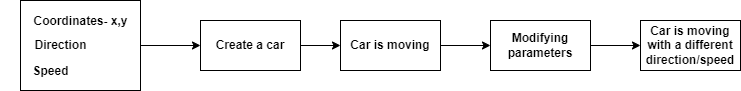
\includegraphics[width=1\textwidth]{images/Arhitecture.png}
    \caption{Architecture of the project}
    \label{fig:rendszer_blokk}
\end{figure}


\subsection{Sequence Diagrams}

\subsubsection{Adding a Vehicle}

The following sequence diagram (fig \ref{fig:add_vehicle_diagram}) illustrates the process of adding a vehicle to the application.


\begin{figure}[h]
    \centering
    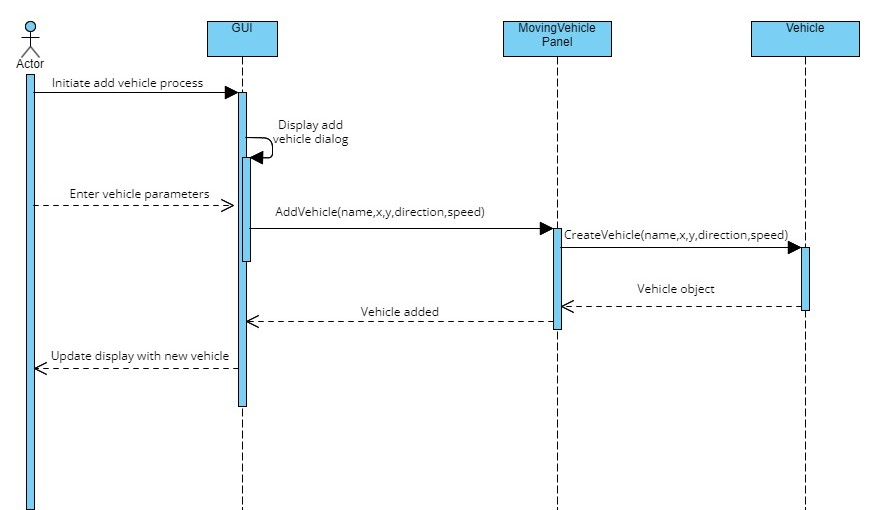
\includegraphics[width=1\textwidth]{images/Add vehicle diagram.jpg}
    \caption{Add vehicle diagram}
    \label{fig:add_vehicle_diagram}
\end{figure}

\newpage
\subsubsection{Moving a Vehicle}

The following sequence diagram (fig \ref{fig:direction_change_diagram})illustrates the process of moving a vehicle in a specific direction.

\begin{figure}[h]
    \centering
    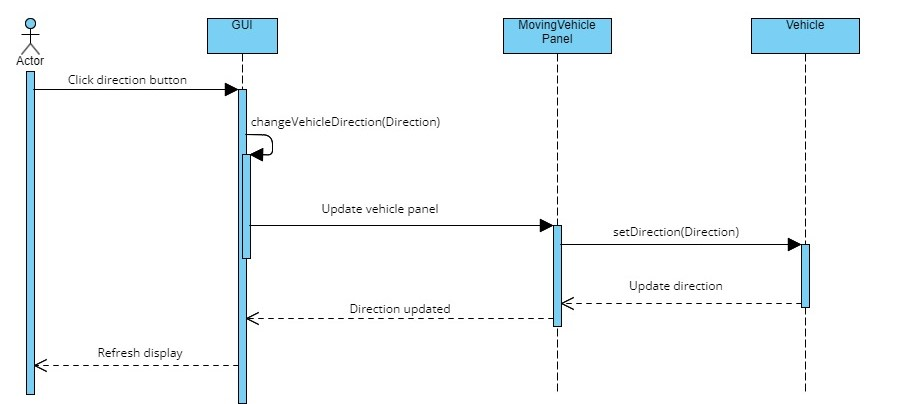
\includegraphics[width=1\textwidth]{images/Direction change diagram.jpg}
    \caption{Direction change diagram}
    \label{fig:direction_change_diagram}
\end{figure}

\section{Class Overview}

\subsection{Main}

\begin{itemize}
    \item Contains the main method, which is executed when the application is launched.
    \item Initializes the main graphical user interface (GUI) by creating an instance of MovingVehicleGUI.
    \item Starts the application and displays the GUI to the user.
\end{itemize}





\subsection{MovingVehicleGUI}

\begin{itemize}
    \item Responsible for managing the main graphical user interface of the application.
    \item Handles user interactions such as adding vehicles, modifying parameters, and moving vehicles.
    \item Interacts with other components such as MovingVehiclePanel and VehicleListWindow to update the UI.
\end{itemize}


\subsection{MovingVehiclePanel}

\begin{itemize}
    \item Represents the canvas where vehicles are displayed and their movements are simulated.
    \item Manages the rendering of vehicles and their movements.
    \item Provides methods for adding vehicles, updating their positions, and performing boundary checks.
\end{itemize}


\subsection{Vehicle}

\begin{itemize}
    \item Represents Represents a single vehicle in the application.
    \item Stores information such as name, coordinates (x, y), direction, and speed of the vehicle.
    \item Provides methods for updating the vehicle's position, changing its direction, and modifying its parameters.

\end{itemize}


\subsection{VehicleListWindow}


\begin{itemize}
    \item Represents Displays a list of all vehicles currently present in the application.
    \item Allows users to select a vehicle from the list and modify its parameters.
    \item Keeps track of changes to the vehicle list and updates the UI accordingly.

\end{itemize}

\section{Conclusion}

I am pleased to announce that I have successfully developed an application featuring moving vehicles. Through planning and implementation, we have created a dynamic and interactive platform that allows users to simulate vehicle movements, modify parameters, and visualize their positions in real-time.

\end{document}
